\documentclass[a5paper, twoside]{article}

%\usepackage{showframe}

%\usepackage[flowers]{../../template}
\usepackage{../../template}
\usetikzlibrary{tikzmark}
\usetikzlibrary{fit}

\usepackage{wrapfig}

\geometry{
%  showframe,
  a5paper, 
  total={124.5mm, 165mm}, 
  top=20mm, 
  marginpar={0mm},
  left={12mm},
  %right={26mm},
  headsep=5mm
}
\tikzcdset{scale cd/.style={every label/.append style={scale=#1},
    cells={nodes={scale=#1}}}}
\pdfcompresslevel=0


\renewcommand{\contentsname}{Spis rozmaitości treściowalnych}

\usepackage{titlesec}
\usepackage[dotinlabels]{titletoc}
\titleformat{\section}[hang]{\color{purple}\sffamily\bfseries\Large}{\color{purple}Wykład }{0.2em}{}
\titlespacing*{\section}{0pt}{2\baselineskip}{1.25\baselineskip}
\titleformat{\subsection}[hang]{\color{purple}\sffamily\bfseries\large}{\color{purple}\thesubsection}{0.4em}{}
\titlespacing*{\subsection}{2em}{1\baselineskip}{1\baselineskip}

\makeatletter %only needed in preamble
\renewcommand\Large{\@setfontsize\Large{12pt}{9}}
\renewcommand\large{\@setfontsize\large{10pt}{9}}
\renewcommand\scriptsize{\@setfontsize\scriptsize{5pt}{5}}
\renewcommand\small{\@setfontsize\small{6pt}{6}}
\makeatother

\fancyhead[LE, RO]{\rightmark}

\setheader{Funkcje analityczne R}
\setfoot{Szwarca}

\fancyfoot[LE, RO]{\color{black!20}\scalefont{0.8} }%Weronika Jakimowicz}

\title{Funkcje analityczne R}
\author{}
\date{Zima 2023-24}


%\includeonly{15:22-01-23.tex}

\begin{document}
\scalefont{0.8}


\maketitle
\thispagestyle{empty} 
\newpage

\tableofcontents
\thispagestyle{empty}
\newpage

\pagestyle{fancy}

\section{20.02.24 : Wprowadzenie do liczb zespolonych}

\subsection{Liczby zespolone jako płaszczyzna}

Liczby zespolone utożsamiamy z płaszczyzną: $(x,y)\iff x+iy$. Możemy wtedy pisać $\C=\R+i\R$. Ponieważ jest to pole wektorowe, to możemy dodawać liczby zespolone i mnożyć je przez liczby rzeczywiste. Dodatkowo, przy założeniu, że przez $i$ oznaczamy abstrakcyjne rozwiązanie równania $x^2+1=0$ (tzn. $i^2=-1$), możemy zdefiniować iloczyn wektorów jako 
$$(x_1, y_1)(x_2, y_2)=(x_1x_2-y_1y_2, x_1y_2+x_2y_1)$$
$$(x_1+iy_1)(x_2+iy_2)=x_1x_2-y_1y_2+i(x_1y_2+x_2y_1)$$
Z dodawaniem oraz iloczynem $\C$ jest ciałem (przemiennym).

Sprawdzamy, czy każdy element naprawdę jest odwracalny. Niech $z=x+iy$, gdzie $x\neq 0$ lub $y\neq 0$. Wtedy
$$\frac{1}{z}=\frac{1}{x+iy}=\frac{x-iy}{x^2+y^2}=\frac{x}{x^2+y^2}+i\frac{-y}{x^2+y^2}.$$

\begin{definition}[część rzeczywista, urojona]
  Jeśli $z=x+iy$ jest liczbą zespoloną, to oznaczamy
  $$x=\Re (z)$$
  co jest \acc{częścią rzeczywistą} liczby $z$ oraz
  $$y=\Im(z)$$
  \acc{część urojona}.
\end{definition}

Chcemy umieć liczyć długość wektorów z $\C=\R+i\R$, czyli definiujemy
\begin{definition}[sprzężenie (moduł)]
  Dla liczby zespolonej $z=x+iy$ piszemy
  $$\overline{z}=x-iy,$$
  co nazywamy \acc{sprzężeniem} liczby $z$. Dzięki temu możemy też zdefiniować \acc{moduł} (długość) liczby zespolonej $z$:
  $$|z|=\sqrt{x^2+y^2}=\sqrt{z\overline{z}}.$$
\end{definition}
Geometrycznie, o sprzężeniu możemy myśleć jako o odbiciu wzdłuż osi $OX$:
\begin{center}
  \begin{tikzpicture}
    \draw[->] (0, 0.5)--(0, 4);
    \draw[->] (-0.5,2)--(4, 2);
    \draw[orange](0,2)--(3.5, 3.5);
    \node at (3, 3.5) {$\color{orange}z$};
    \draw[green](0,2)--(3.5, 0.5);
    \node at (3, 0.5) {$\color{green}\overline{z}$};
  \end{tikzpicture}
\end{center}

\begin{lemma}[własności sprzężenia]
  Dla liczb zespolonych $z_1,z_2$ mamy:
  $$\overline{z_1z_2}=\overline{z_1}\;\overline{z_2}.$$
  Z tego wynika, że $|z_1z_2|=|z_1||z_2|$. Dalej,
  $$\overline{\left(\frac{z_1}{z_2}\right)}=\frac{\overline{z_1}}{\overline{z_2}}$$
  co daje nam $\left|\frac{z_1}{z_2}\right|=\frac{|z_1|}{|z_2|}$.
\end{lemma}

Dla liczb zespolonych zachodzi własność trójkąta, tzn. $|z_1+z_2|\leq |z_1|+|z_2|$, którą dowodzimy podnosząc obie strony do kwadratu:
\begin{align*}
  |z_1+z_2|^2&=(z_1+z_2)(\overline{z_1}+\overline{z_2})=|z_1|^2+z_1\overline{z_2}+\overline{z_1}z_2+|z_2|^2=\\ 
             &=|z_1|^2+z_1\overline{z_2}+\overline{z_1\overline{z_2}}+|z_2|^2=|z_1|^2+2\Re(z_1\overline{z_2})+|z_2|^2\\ 
  (|z_1|+|z_2|)^2&=|z_1|^2+2|z_1||z_2|+|z_2|^2\geq|z_1|^2+2|\Re(z_1\overline{z_2})|+|z_2|^2
\end{align*}

\subsection{Postać trygonometryczna i pierwiastki wielomianów}

\begin{definition}[postać trygonometryczna]
  Niech $z=x+iy$ będzie liczbą zespoloną. Geometrycznie, jest ona reprezentowana przez

  \begin{center}
    \begin{tikzpicture}
      \draw[->](-0.5, 0)--(4, 0);
      \draw[->](0, -0.5)--(0, 4);
      \draw[orange] (0,0)--(60:4);
      \node at (50:4.1) {$x+iy$};
      \node at (65:2) {\rotatebox{60}{$\color{orange}r$}};
      \draw[dashed] (60:4.1)--(0:{4*cos(60)});
      \node at (40:3.08) {$y$};
      \draw (0.5, 0) arc (0:60:0.5);
      \node at (0.6, 0.35) {$\theta$};
    \end{tikzpicture}
  \end{center}

  $$x=r\cos \theta\quad y=r\sin \theta$$
  $$z=x+iy=r(\cos \theta+i\sin \theta).$$
\end{definition}
Wtedy mnożenie liczb zespolonych prezentuje się następująco:
\begin{align*}
  z_1z_2&=r_1(\cos\theta_1+i\sin\theta_2)r_2(\cos\theta_2+i\sin\theta_2)=\\ 
        &=r_1r_2(\cos(\theta_1+\theta_2)+i\sin(\theta_1\theta_2)).
\end{align*}
Możemy to uogólnić na stwierdzenie, że \emph{przy mnożeniu liczb zespolonych mnożymy moduły i dodajemy kąty}.

\begin{example}
  \item Dla ustalonego $z$ chcemy znaleźć $z_0$ takie, że $z_0^n=z$. Korzystając z pierwszej definicji mnożenia lewa strona równania jest potworkiem. Jeśli jednak użyjemy postaci trygonometrycznej wraz ze \buff{wzorem de Moire'a} ($z^n=r^n(\cos(n\theta)+i\sin(n\theta)$), to dostaniemy 
    $$z_0^n=r_0^n(\cos(n\theta_0)+i\sin(n\theta_0))=r(\cos\theta+i\sin\theta)$$
    z czego wnioskujemy, że 
    $$n\theta_0=\theta+2k\pi\implies \theta_0=\frac{\theta}{n}+\frac{2k\pi}{n}$$
    wystarczy rozważać $k=0, 1,..., n-1$.

    Dostajemy więc $n$ różnych rozwiązań równania.
  \item Pierwiastki z $1$ to rozwiązania równania
    $$z^n=1$$
    czyli liczby postaci
    $$z_k=\cos\frac{2k\pi}{n}+i\sin\frac{2k\pi}{n}$$
    dla $k=0,...,n-1$. Jedno z tych rozwiązań jest specjalne, mianowicie
    $$\omega=\cos\frac{2\pi}{n}+i\sin{2\pi}{n},$$
    gdyż jej potęgowanie generuje pozostałe pierwiastki $1$.
\end{example}

\begin{theorem}[Zasadnicze twierdzenie algebry]
  Wielomian 
  $$w(z)=a_nz^n+...+a_1z+a_0,$$
  gdzie $a_n\neq 0$, ma $n$ pierwiastków zespolonych wraz z krotnościami.
\end{theorem}

\begin{proof}
  Żeby udowodnić twierdzenie wyżej wystarczy udowodnić, że wielomian $w(z)$ ma co przynajmniej jeden pierwiastek. Wtedy wielomian rozłoży się na $w(z)=(z-z_1)v(z)$.

  Do dowodu tego twierdzenia wrócimy później.
\end{proof}

\subsection{Funkcje ciągłe}

\begin{definition}[zbieżność ciągu]
  Mówimy, że ciąg $z_n=x_n+iy_n$ jest zbieżny do $z=x+y$, jeśli $x_n\to x$ i $y_n\to y$. Równoważnie, możemy powiedzieć, że 
  $$|z_n-z|\to 0,$$
  co wynika wprost z nierówności trójkąta:
  $$\begin{matrix}|x_n-x|\\|y_n-y|\end{matrix}\leq |z_n-z|\leq |x_n-x|+|y_n-y|.$$
\end{definition}

Rozważmy funkcję $f:\C\to \C$, np. $f(z)=z+1$ czy $f(z)=\frac{1}{z^2+1}$ dla $z\neq -i,i$. W zależności od wygody będziemy zamiennie stosować zapisy
$$f(x, y):=f(x+iy)$$
lub nawet
$$f(x+iy)=u(x, y)+iv(x, y)$$
gdzie $u(x, y)=\Re(f(x, y))$ i $v(x, y)=\Im(f(x, y))$. Na przykład dla funkcji $f(z)=z^2$ funkcja $u(x, y)=x^2-y^2$, a $v(x, y)=2xy$.

  
Korzystając z wiedzy o $\R$, możemy powiedzieć, że funkcja $f:\C\to\C$, $f=u+iv$, jest ciągła jako funkcja zespolona, jeśli jest ciągła jako funkcja z $\R^2$ do $\R^2$. To znaczy, że każda z funkcji $u$ i $v$ jest ciągła. Tak samo funkcja $f$ ma granicę, jeśli $u$ oraz $v$ mają granicę.

\begin{definition}[granica funkcji]
  Nie odwołując się do rozbicia $f$ na $u$ oraz $v$ i napisać, że funkcja $f(z)$ ma pewną granicę $g$ w punkcie $z_0$, jeśli
  $$|f(z)-g|\xrightarrow[z\to z_0]{} 0.$$
\end{definition}

\begin{example}
\item Chcemy przeliczyć
  $$\lim\limits_{z\to i}\frac{z-i}{z^2+1}=\lim\limits_{z\to i}\frac{z-i}{(z-i)(z+i)}=\frac{1}{2i}$$
  ale tutaj rozbiliśmy funkcję na iloczyn dwóch funkcji. Musimy więc udowodnić, że dla liczb zespolonych to naprawdę ma miejsce.
  %i uwierzyliśmy, że
  %$$\lim\limits_{z\to z_0}\frac{f(z)}{g(z)}=\frac{a+bi}{c+di},$$
  %o ile $f\to a+bi$ i $g\to c+di\neq 0$.
\end{example}

\begin{lemma}
  $$\lim\limits_{z\to z_0}\frac{f(z)}{g(z)}=\frac{a+bi}{c+di}$$
  o ile $f\to a+bi$ i $g\to c+di\neq 0$.
\end{lemma}

\begin{proof}
  \begin{align*}
    \frac{f(z)}{g(z)}&=\frac{u_1+iv_1}{u_2+iv_2}=\frac{(u_1+iv_1)(u_2-iv_2)}{u_2^2+v_2^2}=\\ 
                     &=\frac{u_1u_2+v_1v_2}{u_2^2+v_2^2}+i\frac{v_1u_2-v_2u_1}{u_2^2+v_2^2}\to\\ 
                     &\to \frac{ac+bd}{c^2+d^2}+i\frac{bc-ad}{c^2+d^2}=\frac{a+bi}{c+di}.
  \end{align*}
\end{proof}

\begin{definition}[ciągłość funkcji w punkcie]
Mówimy, że $f$ jest ciągła w $z_0$, jeśli $f$ jest określona w pobliżu $z_0$ oraz 
$$\lim\limits_{z\to z_0}f(z)=f(z_0).$$
\end{definition}

Suma, iloczyn i iloraz funkcji ciągłych w $z_0$ są funkcjami ciągłymi w $z_0$. 

\begin{definition}[ciągłość funkcji w obszarze] 
  Funkcja $f$ jest ciągła w obszarze otwartym $U\subseteq \C$ (to samo co obszar otwarty w $\R^2$), jeśli jest ciągła w każdym punkcie z $U$.

  Funkcja $f$ jest ciągła w obszarze $U\subseteq \C$, jeśli jest ciągła w $Int(U)$ oraz dla $z_n\in U$ i $z_n\to z_0\in U$, to $f(z_n)\to f(z_0$.
\end{definition}

\begin{theorem}[Weierstrassa]
  Jeśli $f(z)$ jest ciągła w domkniętym i ograniczonym obszarze $D\subseteq\C$, to $f(z)$ jest ograniczone dla $z\in D$. To znaczy, że istnieje stała $M$ takie, że dla wszystkich $z\in D$ $|f(z)|\leq M$.
\end{theorem}

Nie działa tutaj jednak wersja twierdzenia Weierstrassa o osiąganiu kresów dla funkcji $\R\to\R$, gdyż na $\C$ nie ma dobrego porządku.

\begin{lemma}[ciągłość złożenia]
  Można udowodnić, że jeśli $f(z)$ jest ciągła w $z_0$ oraz $g(w)$ jest ciągła w $w_0=f(z_0)$, to $g\circ f$ jest ciągła w $z_0$.
\end{lemma}

Co wynika z twierdzeń z analizy rzeczywistej.

\subsection{Zadania}

{\large\color{red}WARTO WRÓCIĆ I DOPISAĆ EXPLICITE HOMOTOPIE}

Zakładamy, że wszystkie rozpatrywane przestrzenie topologiczne są drogowo spójne.

\begin{problem}
  Uzasadnij, że składanie dróg spełnia następujący warunek skreśleń: jeśli $f_0g_0\sim f_1g_1$ oraz $g_0\sim g_1$, to $f_0\sim f_1$.
\end{problem}

\begin{solution}
  Niech $g_0$ będzie drogą o początku w $x_0$. Zauważmy, że podobnie jak w pętlach
  $$f_0\sim f_0 x_0\sim f_0(g_0g_0^{-1})\sim (f_0g_0)g_0^{-1}.$$
  Wiemy, że $(f_0g_0)\sim f_1g_1$. Z drugiej strony, skoro $g_0\sim g_1$, to idąc "od tyłu" po homotopii między tymi drogami, tzn. $G'(s, t)=G(1-s, t)$, dostajemy homotopię między $g_0^{-1}$ a $g_1^{-1}$. Czyli
  $$f_0\sim f_0x_0\sim (f_0g_0)g_0^{-1}\sim (f_1g_1)g_1^{-1}\sim f_1(g_1g_1^{-1})\sim f_1x_0\sim f_1$$
\end{solution}

\begin{problem}
  Pokaż bezpośrednio z definicji, że dla pętli $f,g$ w $X$ zbazowanych w $x_0\in X$ zachodzi równoważność $f\sim g\iff f g^{-1}\sim x_0$, gdzie $x_0$ to pętla stała zbazowana w $x_0$, zaś $g^{-1}$ to pętla odwrotna do $g$.
\end{problem}

\begin{solution}
  $\implies$
  
  Zaczynamy od napisania homotopii 
  $$fg^{-1} \sim gg^{-1},$$ 
  czyli funkcji
  $$G(s, t)=H(s, 1-t)g(1-s).$$ 
  Potem, korzystając ze wzoru w dowodzie twierdzenia \ref{twierdzenie:1.4} dostajemy homotopię $gg^{-1}\sim x_0$. To daje nam 
  $$fg^{-1}\sim gg^{-1}\sim x_0$$ 
  tak jak chcieliśmy.

  $\impliedby$

  Niech $H(s, t)$ będzie homotopią między $fg^{-1}$ a $x_0$. Wtedy $H(s, t)g(s)$ będzie homotopią między $fg^{-1}g$ a $x_0g$, co po skorzystaniu ze wzoru użytego w twierdzeniu \ref{twierdzenie:1.4} daje
  $$f\sim fg^{-1}g\sim x_0g.$$
  Pozostaje napisać homotopię $x_0g\sim g$. Będzie to funkcja stale równa $x_0$ na odcinku $[0, (1-t)/2]$ oraz $g(s)$ na pozostałej długości przedziału $[0,1]$. Wzorem, wygląda to następująco:
  $$G(s, t)=\begin{cases}
  x_0&s\leq \frac{1-t}{2}\\ g\left(\left(s-\frac{1-t}{2}\right)\frac{2}{1+t}\right)&\frac{1-t}{2}<s\end{cases}$$
\end{solution}

\begin{problem}
  Uzasadnij, że dla dowolnej przestrzeni topologicznej $X$ następujące trzy warunki są równoważne:
  \begin{enumerate}[label=\alph*)]
    \item każde odwzorowanie $S^1\to X$ jest homotopijne ze stałym
    \item każde odwzorowanie $S^1\to X$ rozszerza się do odwzorowania $D^2\to X$, gdzie $D^2$ to $2$-wymiarowy dysk, którego brzegiem jest nasze $S^1$
    \item $\pi_1(X, x_0)=0$ dla dowolnego $x_0\in X$
  \end{enumerate}
  Wywnioskuj stąd, że przestrzeń $X$ jest jednospójna wtedy i tylko wtedy gdy wszystkie odwzorowania $S^1\to X$ są homotopijne.
\end{problem}

\begin{solution}
  $a)\implies b)$

  Utożsamimy $S^1$ z okręgiem jednostkowym na płaszczyźnie, czyli zbiorem punktów 
  $$\{(\cos\theta, \sin\theta)\;:\;\theta\in[0,2\pi)\}.$$
  Wtedy $D^2$ to zbiór
  $$\{(r\cos\theta, r\sin\theta)\;:\;\theta\in[0,2\pi), 0\leq r\leq 1\}=S^1\times [0,1]/ S^1\times\{0\}.$$
  Niech teraz $H(t, s)$ będzie homotopią między $f$ a odwzorowaniem stałym $c$. Wtedy
  $$F:D^2=S^1\times[0,1]/S^1\times\{0\}\to X$$
  jest zdefiniowane jako 
  $$F(s, t)=H(s, t)=f_t(s)$$

  $b)\implies a)$

  Weźmy dowolne odwzorowanie $f:S^1\to X$. Z $b)$ wiemy, że możemy je "zakleić". Niech $F:S^1\times [0,1]/S^1\times\{0\}=D^2\to X$ będzie rozszerzeniem $f$, dla którego $F(0,1)=x_1$, $F(x, 1)=f(x)$ oraz $F(x, 0)=c$ jest stałe niezależnie od wyboru $x$. 

  Napiszmy odwzorowanie 
  $$H(s, t)=F(s, 1-t),$$
  które jest homotopią między $f$ a "środkiem" dysku $c$. Jest to więc homotopia między odwzorowaniem $f$ a funkcją stale równą $c$.
  %Wystarczy tylko dodać tutaj odwzorowanie, które w sposób ciągły $F(0, 0)=c$ przesuwa na $F(0, 1)=x_0$. 

  $c)\implies a)$

  Dowolna pętlę możemy zinterpretować jako odwzorowanie $f:S^1\to X$. Niech $x_0=f(0)$. Z $c)$ wiemy, że $\pi_1(X, x_0)=0$, czyli $[x_0]=[f]$ i $f$ jest homotopijne z odwzorowaniem stale równym $x_0$.

  $a)\implies c)$

  Wybierzmy dowolne $x_0\in X$. Niech $f:S^1\to X$ będzie dowolnym odwzorowaniem takim, że $f(0)=f(1)=x_0$. Wiemy, że jest ono homotopijne z odwzorowaniem stałym $f\sim c$. Wystarczy teraz zauważyć, że homotopia między $f$ a $c$ daje również homotopię między $c$ a $x_0$. Czyli dowolna pętla $f:S^1\to X$ zbazowana w $x_0$ jest homotopijna z $x_0$. Stąd $\pi_1(X, x_0)=0$ dla dowolnego $x_0$.

  \begin{center}
    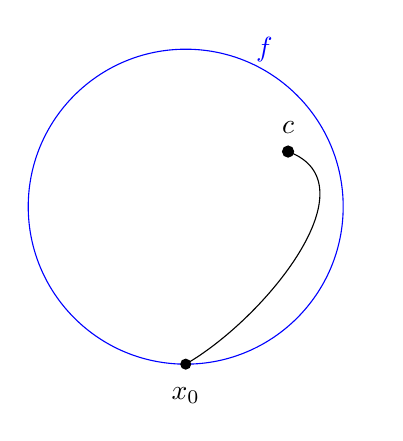
\begin{tikzpicture}
      \draw[blue] (0,0) circle (2);
      \fill (0, -2) circle (2pt);
      \draw (1.3, 0.7) circle (2pt);
      \draw (0,-2) to [out=30, in=-20] (1.3, 0.7);
      \fill (1.3, 0.7) circle (2pt);
      \node at (1.3, 1) {$c$};
      \node at (0,-2.4) {$x_0$};
      \node at (1, 2) {$\color{blue}f$};
    \end{tikzpicture}
  \end{center}

  Przestrzeń $X$ jest jednospójna, gdy jest drogowo spójna i ma trywialną grupę podstawową. Jednospójność w oczywisty sposób implikuje warunek $c)$ wyżej, z którego dostajemy, że dowolne dwa odwzorowania $S^1\to X$ są homotopijne z punktami stałymi, które możemy połączyć ($X$ łukowo spójne). 

  Z drugiej strony, jeśli dowolne dwa odwzorowania $S^1\to X$ są homotopijne, to w szczególności każde takie odwzorowanie jest homotopijne z odwzorowaniem stałym $x_0$ dla dowolnego $x_0\in X$. To daje łukową spójność $X$ oraz trywialność grupy podstawowej.
\end{solution}

\begin{problem}
  Jeśli $\pi_1X=0$, to każde dwie drogi łączące dowolnie wybrane dwa punkty $x_0, x_1\in X$ są homotopijne.
\end{problem}

\begin{solution}
  Niech $f, g$ będą drogami między $x_0$ a $x_1$. Wtedy $fg^{-1}$ będzie pętlą zbazowaną w $x_0$. Ponieważ $\pi_1X=0$, to $fg^{-1}\sim x_0$. Z zadania 2 wiemy, że wtedy $f\sim g$.
\end{solution}

\begin{problem}
  Mówimy, że przestrzeń topologiczna $X$ jest ściągalna, jeśli istnieje odwzorowanie $F:X\times I\to X$ takie, że $F(x, 0)=x$ oraz $F(x, 1)=x_0$ dla dowolnego $x$ oraz pewnego ustalonego $x_0$. Uzasadnij, że jeśli $X$ jest przestrzenią ściągalną, to jest też drogowo spójna, oraz $\pi_1X=0$ (innymi słowy, $X$ jest wtedy jednospójna).
\end{problem}

\begin{solution}
  Niech $x_1,x_2\in X$ będą dowolnymi punktami. Wówczas droga $f(t)=F(x_1, t)$ idzie z $x_1$ do $x_0$, a droga $g(t)=F(x_2, 1-t)$ idzie od $x_0$ do $x_2$. Łącząc obie te drogi dostajemy ścieżkę $x_1$ do $x_2$, czyli przestrzeń jest łukowo spójna.

  Weźmy teraz dowolną pętlę $f$ zbazowaną w punkcie $x_0$. Rozważmy homotopię $H(s, t)=F(f(s), t)$, która dla $t=0$ wynosi $f(s)$, a dla $t=1$ jest stale równa $x_0$. Z tego wynika, że $f\sim x_0$, czyli każda pętla jest homotopijna z elementem neutralnym $\pi_1X$ i grupa ta jest trywialna.
\end{solution}

\begin{problem}
  Uzasadnij, że każdy wypukły podzbiór w $\R^n$ jest ściągalny.
\end{problem}

\begin{solution}
  Wybierzmy dowolny punkt $x_0$ i z definicji zbioru wypukłego odcinek łączący $x_0$ z dowolnym innym punktem tego zbioru musi być zawarty w całości w tym zbiorze. Wystarczy napisać funkcję, która w sposób ciągły będzie przesuwać punkty po odcinkach łączących je z $x_0$.
\end{solution}

\begin{problem}
  Niech $T$ będzie skończonym \emph{drzewem}, tzn. spójnym skończonym grafem niezawierającym zamkniętych cykli krawędzi. Uzasadnij, że $\pi_1T=0$.
\end{problem}

\begin{solution}
  Jedyne pętle jakie znajdziemy w $T$ to pętla stała oraz pętle, które idą po wierzchołkach w jedną stronę i wracają po swoich śladach do punktu zaczepienia. Ten drugi rodzaj pętli to $ff^{-1}$ i jest homotopijne równy drodze stałej.
\end{solution}

\begin{problem}
  Uzasadnij, że homomorfizm $\phi_c:\pi_1(X, x_0)\to \pi_1(X, x_1)$ (związany ze zmianą punktu bazowego) zależy tylko od klasy homotopii drogi $d$ od $x_0$ do $x_1$.
\end{problem}

 


\end{document}
